\documentclass[a4paper,twoside,openany]{book}
%\documentclass[aps,prl,preprint,groupedaddress]{revtex4}
%\documentclass[prl,nobibnotes,superscriptaddress,prb]{revtex4}
%%%%%%%%%%%%%%%%%%%%%%%%%%%%%%%%%%%%%%%%%%%%%%%%%%%%%%%%%%%%%%%%%%%%%%%%%%%%%%%%%%%%%%%%%%%%%%%%%%%%%%%%%%%%%%%%%%%%%%%%%%%%
\usepackage{amsmath}
\usepackage{amssymb,graphicx}
%\usepackage{apstemplate}
%TCIDATA{OutputFilter=LATEX.DLL}F
%TCIDATA{Created=Fri Aug 09 14:28:03 2002}
%TCIDATA{LastRevised=Tue Feb 25 19:27:19 2003}
%TCIDATA{<META NAME="GraphicsSave" CONTENT="32">}
%TCIDATA{<META NAME="DocumentShell" CONTENT="Journal Articles\REVTeX - APS and AIP Article">}
%TCIDATA{CSTFile=revtxtci.cst}
\newcommand{\tbf}{\boldsymbol}
%\input{tcilatex}

\textwidth=14cm
\textheight=20cm

\bibliographystyle{plain}
\begin{document}
\begin{titlepage}
\begin{centering}
\vspace*{5cm}

\LARGE
{\bf User manual for the SCPH -program}


\vspace{1cm}

by

Petros Souvatzis

\vspace{1cm}

Department of Physics

\vspace{1cm}
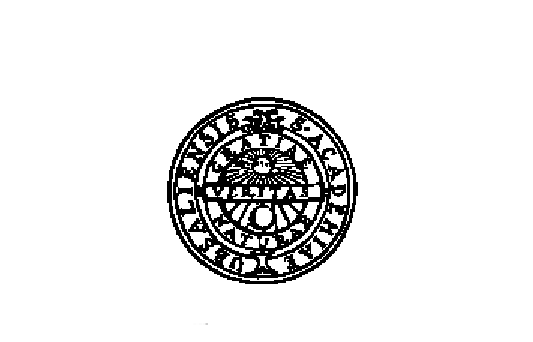
\includegraphics[scale=0.8]{UU_logo}

Uppsala University 2008

\end{centering}
\end{titlepage}

%\newpage

\tableofcontents

\chapter{Introduction}
In this manual/user guide describes how to operate the scph-program in which the self consistent ab initio lattice dynamical method has 
been implemented (SCAILD) \cite{petros}. The program is written in a way  so that it can be easily be interfaced with the VASP package \cite{VASP},
and with the phon-program of Dario Alfe \cite{Dario}. Those of you who have used VASP and phon will thus find it a "peace of cake" to learn how to
use the scph package.

There are also three different directories accompanying this manual 
with all the input files needed to do three different SCAILD calculations. These directories are \texttt{examples/bcc\_Ti/}, \texttt{examples/hcp\_Ti/} and \texttt{examples/CsI/} and
it might be a good idea to take a look at  these files when reading this manual.

%===========================^M
\chapter{Theoretical Background}
%===========================^M
Self consistent phonon calculations are a natural extension of the theory of the
harmonic lattice, and we initiate our methodological description by first presenting the most important features of this theory. The 
Hamiltonian of lattice dynamical system can be expressed as
\begin{equation}\label{eq:E1}
\mathcal{H} = \mathcal{H}_{h} +\mathcal{V}_{anh}
\end{equation}
where
\begin{equation}\label{eq:E2}
\mathcal{H}_{h} = \sum_{\tbf{R},\sigma}\frac{\tbf{P}^{2}_{\tbf{R}\sigma}}{2M_{\sigma}}
+\frac{1}{2}\sum_{\tbf{R},\sigma}\sum_{\tbf{R'},\sigma '}\tbf{U}_{\tbf{R}\sigma}\bar{\bar{\Phi}}^{\sigma\sigma'}
(\tbf{R}+\tbf{b}_{\sigma}-\tbf{R'}-\tbf{b}_{\sigma'})\tbf{U}_{\tbf{R'}\sigma'},
\end{equation}
\begin{eqnarray}
\mathcal{V}_{anh}=\frac{1}{3!}\sum_{\tbf{R},\sigma}\sum_{\tbf{R'},\sigma '}\sum_{\tbf{R''},\sigma ''}\sum_{\alpha \beta \gamma }
\Phi_{\alpha \beta \gamma }^{\sigma\sigma'\sigma''}(\tbf{R}+\tbf{b}_{\sigma},\tbf{R'}+\tbf{b}_{\sigma'},\tbf{R''}+\tbf{b}_{\sigma''})
U_{\tbf{R}\sigma\alpha}U_{\tbf{R'}\sigma'\beta}U_{\tbf{R''}\sigma''\gamma} + \cdots, \nonumber \\ \label{eq:E3}
\end{eqnarray}
are the harmonic and anharmonic parts of the Hamiltonian, respectively.
Here $\mathbf{R}$ are the
equilibrium lattice positions of the atoms, $\mathbf{b}_{\sigma}$ the atomic positions relative to the primitive Bravais lattice,
$\mathbf{U}_{\mathbf{R}\sigma}$ the displacements of the atoms,
$\mathbf{P}_{\mathbf{R}\sigma}$ the momentum of the atoms, $M_{\sigma}$ the
atomic mass, $\bar{\bar{\Phi}}^{\sigma\sigma'}$ the inter-atomic force constant
matrices and $\Phi_{\alpha,\beta,\gamma}^{\sigma\sigma'\sigma''}$ the tensor describing the third order anharmonic contribution to the
potential energy. In order to make the notation more transparent, in the following sections the notation of a monoatomic lattice will be
adapted without any loss of generality.
%%%%%%%%%%%%%%%%%%%
\section{The harmonic lattice and its limitations}
%%%%%%%%%%%%%%%%%%%
Diagonalizing the dynamical matrix
\begin{equation}\label{eq:E4}
\bar{\bar{\mathcal{D}}}(\mathbf{k}) = \frac{1}{M}\sum_{\mathbf{R}}\bar{\bar{\Phi}}(\mathbf{R})e^{-i\mathbf{k}\mathbf{R}},
\end{equation}
for each wave vector $\mathbf{k}$ in the first Brillouin zone one
finds the eigenvalues $\omega_{\mathbf{k}s}$ and eigenvectors
$\mathbf{\epsilon}_{\mathbf{k}s}$ of different phonon modes
(longitudinal or transverse) labeled by the symbol $s$, $N$ being
the number of atoms. Introducing the canonical phonon coordinates
$\mathcal{Q}_{\mathbf{k}s}$ and $\mathcal{P}_{\mathbf{k}s}$, the displacements $\mathbf{U}_{\mathbf{R}}$ and the 
kinetic energy operators $\mathbf{P}_{\mathbf{R}}$ can be expressed as
\begin{eqnarray}
\mathbf{U}_{\mathbf{R}} = \frac{1}{\sqrt{MN}}\sum_{\mathbf{k},s}\mathcal{Q}_{\mathbf{k}s}\mathbf{\epsilon}_{\mathbf{k}s}e^{i\mathbf{k}\mathbf{R}} \label{eq:E5} \\
\mathbf{P}_{\mathbf{R}} =
\frac{1}{\sqrt{MN}}\sum_{\mathbf{k},s}\mathcal{P}_{\mathbf{k}s}\mathbf{\epsilon}_{\mathbf{k}s}e^{i\mathbf{k}\mathbf{R}}
\label{eq:E6}
\end{eqnarray}
allowing a separation of the harmonic Hamiltonian $\mathcal{H}_{h}$ of the crystal
into the Hamiltonians of $3N$ independent harmonic oscillators.
\begin{equation}\label{eq:E7}
\mathcal{H}_{h} = \sum_{\tbf{k}s}\frac{1}{2}( \mathcal{P}_{\mathbf{k}s}^{2}+\omega_{\tbf{k}s}^{2}\mathcal{Q}_{\mathbf{k}s}^{2}).
\end{equation}
The thermodynamic average of the operators
$\mathcal{Q}^{\dagger}_{\mathbf{k}s}\mathcal{Q}_{\mathbf{k}s}$
determines the mean-square atomic displacements and is given by
\begin{equation}
\langle \mathcal{Q}^{\dagger}_{\mathbf{k}s}\mathcal{Q}_{\mathbf{k}s} \rangle =
\frac{\hbar}{\omega_{\mathbf{k}s}}\Big [ \frac{1}{2} + n \Big
(\frac{\hbar\omega_{\mathbf{k}s}}{k_{B}T} \Big ) \Big ],
\label{eq:E8}
\end{equation}
where $n(x) = 1/( e^{x}-1)$ is the Planck function. In the
classical limit, i.e for sufficiently high temperatures, the
operators $(1/\sqrt{M})\mathcal{Q}_{\mathbf{k}s}$ are
replaced by real numbers,
\begin{equation}\label{eq:E9}
\mathcal{R}_{\mathbf{k}s} \equiv \pm
\sqrt{\frac{\langle \mathcal{Q}^{\dagger}_{\mathbf{k}s}\mathcal{Q}_{\mathbf{k}s} \rangle}{M}}.
\end{equation}

Calculating the gradient of the potential energy in Eqn. (\ref{eq:E2}) with respect to the atomic 
displacements gives
the restoring force
\begin{equation}\label{eq:E10}
\mathbf{F}_{\mathbf{R}}= - \sum_{R'}\bar{\bar{\Phi}}(\mathbf{R}-\mathbf{R}')\mathbf{U}_{\mathbf{R}'}.
\end{equation}
Fourier transforming Eqn.(\ref{eq:E10}) and substituting $\mathbf{U}_{\mathbf{R}}$ with the expression in Eqn. (\ref{eq:E5}) 
gives
\begin{equation}\label{eq:E11}
\mathbf{F}_{\mathbf{k}} = -\sum_{s}M\omega_{\mathbf{k}s}^{2}\mathcal{R}_{\mathbf{k}s}\mathbf{\epsilon}_{\mathbf{k}s}.
\end{equation}
Finally, using the orthogonality of the eigenvectors $\epsilon_{{\bf k}s}$ the phonon frequencies can be expressed as
\begin{equation}\label{eq:E12}
\omega_{\mathbf{k}s} = \Big [ -\frac{1}{M}\frac{ \mathbf{\epsilon}_{\mathbf{k}s}\mathbf{F}_{\mathbf{k}}}{\mathcal{R}_{\mathbf{k}s}} \Big ]^{1/2}.
\end{equation}

The equations discussed so far can be solved for dynamically stable materials, where the excitation of any individual phonon mode, i.e a finite  $\mathcal{Q}_{\mathbf{k}s}$, 
will lead to an increase of the total energy $E_{tot}$ of the system, i.e $dE_{tot}/d\mathcal{Q}_{\mathbf{k}s} \ge 0$.
 For dynamically unstable materials however, there exists one or several phonon modes $(\mathbf{k},s)$ such that any
   finite $\mathcal{Q}_{\mathbf{k}s}$ for these modes will result in a decrease in the total energy of the lattice.
In this situation the equations discussed so far can not be used straight forwardly since they result in imaginary phonon frequencies.
 This represents a situation where the lattice under consideration spontaneously shifts atomic planes and/or atomic positions so that 
a new crystal structure lowers the total energy.
 
The only type of anharmonicity that can be taken into account by the above formalism is the type of anharmonicity responsible for the thermal expansion.
This is a weaker kind of anharmonicity that most people are aware of is present in all solids.  Qualitatively it can be described by the simple argument that  longer bonds are
weaker, so the frequencies are lower, so the entropy is higher. To capture the anharmonicity associated to the thermal expansion quasiharmonic DFT works very well. Here the change of
phonon frequencies is almost entirely due to thermal expansion. However, whenever strong anharmonicity appears quasiharmonic phonons may show unstable modes which cannot be stabilized by the thermal expansion. Thus  the interaction between phonons must be included in order to correctly describe the lattice dynamics of the systems. In the following section it will be explained  how the interaction between phonons can been taken into account by means of the SCAILD method.
%
\section{The SCAILD method}
%
To understand how the SCAILD incorporates the effect of anharmonicity in the calculations of phonon frequencies
it is instructive to substitute the lattice displacements in the Hamiltonian (\ref{eq:E1}) with the decomposition
of $U_{\mathbf{R}}$ given by Eqn. (\ref{eq:E5}), to obtain the following expression for the Hamiltonian
\begin{eqnarray}
\mathcal{H}=  
\frac{1}{2}\sum_{\tbf{k}s}\Big [ \mathcal{P}_{\mathbf{k}s}^{2}+ 
\omega_{\tbf{k}s}^{2}
\Big ( 1  + \frac{1}{3}\sum_{\tbf{k}_{1},\tbf{k}_{2}}\sum_{s_{1},s_{2}}\mathcal{A}(\tbf{k},\tbf{k}_{1},\tbf{k}_{2},s,s_{1},s_{2})
\frac{\mathcal{Q}_{\tbf{k}_{1}s_{1}}\mathcal{Q}_{\tbf{k}_{2}s_{2}}}{\mathcal{Q}_{\tbf{k}s}\omega_{\tbf{k}s}^{2}}+
\cdots \Big )\mathcal{Q}_{\tbf{k}s}^{2} \Big ] 
\label{eq:E13} 
\end{eqnarray}
where
\begin{eqnarray}
\mathcal{A}(\tbf{k},\tbf{k}_{1},\tbf{k}_{2},s,s_{1},s_{2})= \qquad \qquad \qquad \qquad \qquad \qquad \qquad \qquad \qquad \qquad \qquad\nonumber \\
\frac{1}{(MN)^{3/2}}\sum_{\tbf{R},\tbf{R}_{1},\tbf{R}_{2}}\sum_{\alpha,\beta,\gamma}
\Phi_{\alpha\beta\gamma}(\tbf{R},\tbf{R}_{1},\tbf{R}_{2})\tbf{\epsilon}_{\tbf{k}s\alpha}\tbf{\epsilon}_{\tbf{k}_{1}s_{1}\beta}
\tbf{\epsilon}_{\tbf{k_{2}}s_{2}\gamma}e^{i(\tbf{Rk}+\tbf{R}_{1}\tbf{k}_{1}+\tbf{R}_{2}\tbf{k}_{2})}  \label{eq:E14}
\end{eqnarray}
The full Hamiltonian of Eqn. (\ref{eq:E13}) is contrary to the Harmonic problem not separable into $N$ independent
Hamiltonians. Nevertheless by replacing the operators $\mathcal{Q}_{\tbf{k}s}$ 
appearing in the curved brackets of Eqn. (\ref{eq:E13}) with $\sqrt{M}\mathcal{R}_{\tbf{k}s}$ the following 
mean-field Hamiltonian can be constructed
\begin{equation}\label{eq:E15}
\mathcal{H}^{MF} = \sum_{\tbf{k}s}\frac{1}{2}(  \mathcal{P}_{\mathbf{k}s}^{2}+\bar{\omega}_{\tbf{k}s}^{2}\mathcal{Q}_{\tbf{k}s}^{2} )
\end{equation}
where
\begin{eqnarray}
\bar{\omega}_{\tbf{k}s}^{2}= \omega_{\tbf{k}s}^{2}\Big (1+   %\qquad  \qquad  \qquad  \qquad  \qquad \qquad  \qquad  \nonumber \\ 
\frac{\sqrt{M}}{2}\sum_{\tbf{k}_{1},\tbf{k}_{2}}\sum_{s_{1},s_{2}}\mathcal{A}(\tbf{k},\tbf{k}_{1},\tbf{k}_{2},s,s_{1},s_{2})
\frac{\mathcal{R}_{\tbf{k}_{1}s_{1}}\mathcal{R}_{\tbf{k}_{2}s_{2}}}{\mathcal{R}_{\tbf{k}s}\omega_{\tbf{k}s}^{2}}+
\cdots \Big ) \label{eq:E16}
\end{eqnarray}
The set of equations \ref{eq:E8}-\ref{eq:E9} and \ref{eq:E15}-\ref{eq:E16} can, once the interaction terms
$\mathcal{A}(\tbf{k},\tbf{k}_{1},\tbf{k}_{2},s,s_{1},s_{2}),$ and an initial guess in terms of normal modes
have been provided, be solved self consistently.

It follows from experience of calculations of anharmonic effects in metals \cite{ktsn1,ktsn2} that
usually odd-order terms are dominant for close packed stiff lattices, such as Ir metal \cite{ktsn1}.
At the same time, soft-mode phonon behavior in essentially anharmonic bcc metals, such as Ca
and Sr, is determined by the even-order terms \cite{ktsn2}. The phonon damping is connected
mainly with three-phonon processes and cannot be taken into account in the framework of
self-consistent phonon picture. In this sense, our approach is reminiscent the quasiparticle
self-consistent GW approximation \cite{GW} where only real part of the electron self-energy is taken
into account.

In the SCAILD scheme Equations (\ref{eq:E8})-(\ref{eq:E9}) and (\ref{eq:E15})-(\ref{eq:E16}) 
are solved by first calculating a starting guess for the phonon dispersions by means
of a standard supercell calculation, see e.g Ref. \cite{PETROS}.
The phonon frequencies corresponding to k-vectors commensurate with the supercell
are then used to calculate the atomic displacements through Eqn. (\ref{eq:E5}) and Eqns. (\ref{eq:E8})-(\ref{eq:E9}). Here it should be noted 
that the signs of the amplitudes $\mathcal{A}_{{\bf k}s}$ (see Eqn.(\ref{eq:E9})), should be chosen randomly, with 
equal probabilities for + and -. It should also be stressed that in the first iterations of the calculation unstable modes may be present,  i.e there may be modes with $\omega_{\tbf{k}s}^{2}< 0$. In order to calculate the Fourier amplitude $\mathcal{R}_{{\bf k}s}$ for these modes by means Eqns. (\ref{eq:E8})-(\ref{eq:E9}) the frequencies have to 
be guessed. In these situations the absolute value $|\omega_{\tbf{k}s}|$ of the imaginary frequencies have been used as guesses of the real frequencies. 

The forces induced
by the displacements $U_{\bf R}$ can be calculated by any standard ab initio method. From the Fourier transform
of the atomic forces a new set of frequencies $\bar{\omega}_{\tbf{k}s}^{2}$ are calculated through Eqn. (\ref{eq:E12})
(in the appendix we describe how one from Eqn. (\ref{eq:E12}) can extract $\bar{\omega}_{\tbf{k}s}^{2}$)
The symmetries of
the different k-vectors are restored by
\begin{equation}\label{eq:symm}
\Omega_{\mathbf{k}s}^{2}= \frac{1}{m_{\mathbf{k}}}\sum_{\mathcal{S}\in \mathcal{S}(\mathbf{k})}\bar{\omega}_{\mathcal{S}^{-1}\mathbf{k}S}^{2},
\end{equation}
where $\mathcal{S}(\mathbf{k})$ is the symmetry group of the wave
vector $\mathbf{k}$, and $m_{k}$ the number of elements of the
group. The mean value of all iterations supplies a new set of
frequencies,
\begin{equation}\label{eq:mean}
\omega_{\mathbf{k}s}^{2}(N_{I})= \frac{1}{N_{I}}\sum_{i=1}^{N_{I}}\Omega_{\mathbf{k}s}^{2}(i),
\end{equation}
where  $\Omega_{\mathbf{k}s}(i)$, $i=1,...,N_{I}$ are the symmetry
restored frequencies from all iterations.  Here $N_{I}$ is the number of iterations. The new set of
frequencies calculated in (\ref{eq:mean}) determine a new set of
displacements used to calculate a new set of forces. 
In Fig. \ref{fig:scematics} a schematic outline is shown of the different steps performed in a SCAILD calculation.
\begin{figure*}[tbp]
\begin{center}
\includegraphics*[angle=0,scale=0.35]{figs/Fig2_thesis}
\caption{(color online).  Schematic outline over the different tasks performed in a self-consistent phonon calculation.}
\label{fig:scematics}
\end{center} 
\end{figure*}
Philosophically our approach is similar to Born's self consistent phonon theory, with the main difference being that we consider 
a direct force calculation from a super cell with Hellman-Feynman forces calculated from density functional  theory.
\newpage
\section{Theoretical appendix}
This appendix shows how the eigenvalues $\bar{\omega}_{\mathbf{k}s}^{2}$ of the mean 
field Hamiltonian (\ref{eq:E15}) can be retained from Eqn. ({\ref{eq:E12}).
Using the sum convention for the coordinate indexes the forces can be expressed as
%
\begin{eqnarray}
F_{\tbf{R}j} = -\sum_{\tbf{R}'}\bar{\bar{\Phi}}_{j\alpha}(\tbf{R}-\tbf{R}')U_{\tbf{R}'\alpha} %\nonumber \\
-\frac{1}{2}\sum_{\tbf{R}',\tbf{R}''}\Phi_{j\alpha \beta}(\tbf{R},\tbf{R}',\tbf{R}'')U_{\tbf{R}'\alpha}U_{\tbf{R}''\beta}+ \cdots
\end{eqnarray}
%
By replacing the operators $\mathcal{Q}_{\mathbf{k}s}/ \sqrt{M}$ with the real numbers $\mathcal{A}_{\mathbf{k}s}$ in 
the normal mode expansion of $\tbf{U}_{\mathbf{R}}$, the Fourier transform of the forces can be expressed as
\begin{eqnarray}
F_{\tbf{k}j}=-\sum_{s}M\omega_{\tbf{k}s}^{2}\epsilon_{\tbf{k}sj}\mathcal{R}_{\tbf{k}s}
-\frac{1}{2N^{3/2}}\sum_{\tbf{k}_{1},\tbf{k}_{2}}\sum_{s_{1},s_{2}}\Phi_{j\alpha \beta}(\tbf{k},\tbf{k}_{1},\tbf{k}_{2})
\epsilon_{\tbf{k}_{1}s_{1}\alpha}\epsilon_{\tbf{k}_{2}s_{2}\beta}\mathcal{R}_{\tbf{k}_{1}s_{1}}\mathcal{R}_{\tbf{k}_{2}s_{2}}+ \cdots. \nonumber \\ \label{eq:hassse}
\end{eqnarray}
Finally multiplying (\ref{eq:hassse}) with $-\epsilon_{\tbf{k}sj}/(\mathcal{R}_{\tbf{k}s}M)$ and summing over $j$ gives
%
\begin{eqnarray}
-\frac{\tbf{F}_{\tbf{k}}\tbf{\epsilon}_{\tbf{k}s}}{M\mathcal{R}_{\tbf{k}s}}= \omega_{\tbf{k}s}^{2}
\Big ( 1+  %\qquad \qquad \qquad \qquad \qquad \qquad \nonumber \\ 
\frac{\sqrt{M}}{2}\sum_{\tbf{k}_{1},\tbf{k}_{2}}\sum_{s_{1},s_{2}}\mathcal{A}(\tbf{k},\tbf{k}_{1},\tbf{k}_{2},s,s_{1},s_{2})
\frac{\mathcal{R}_{\tbf{k}_{1}s_{1}}\mathcal{R}_{\tbf{k}_{2}s_{2}}}{\mathcal{R}_{\tbf{k}s}\omega_{\tbf{k}s}^{2}}+
\cdots \Big ). \nonumber \\
\label{eq:harald}
\end{eqnarray}
%
where $\mathcal{A}(\tbf{k},\tbf{k}_{1},\tbf{k}_{2},s,s_{1},s_{2})$ is given by (\ref{eq:E14}). Now from \ref{eq:harald} becomes obvious
that the left hand side of (\ref{eq:E12}) is equivalent to $\bar{\omega}_{\mathbf{k},s}$.

\chapter{Setting up a SCAILD calculation}
In order to set up a SCAILD calculation one needs, apart from the scph-program, a first principles program that can calculate inter-atomic 
forces. Any first principles program can of course be used for this purpose, however since the input- and output-format of the scph-program 
follows that of VASP, it will be assumed in this manual that the ab initio program is VASP. 
The scph-program and the ab initio program are interfaced by means of a simple shell script. The structure of the script is the same as the structure found in 
the schematic picture presented in Fig. \ref{fig:scematics}. Translating this picture into a simple bash script one would obtain the following: 
(Observe that the small numbers to the right of each active line of the script are not part of the script, they are just used for reference)\\ \\
\texttt{\#!/bin/sh} \\
\texttt{\#First displacement }\\
\texttt{cp POSCAR\_START1 POSCAR}         $^{_{1}}$\\
\texttt{./vasp}  $^{_{2}}$\\
\texttt{./force\_extract}    $^{_{3}}$ \\
\texttt{cp FORCESI KRAFTER.1}   $^{_{4}}$  \\ \\
$\cdots$ \\ \\
\texttt{\#n:th displacement }  \\
\texttt{cp POSCAR\_STARTn POSCAR}  $^{_{5}}$  \\
\texttt{./vasp}  $^{_{6}}$  \\
\texttt{./force\_extract}  $^{_{7}}$  \\
\texttt{cp FORCESI KRAFTER.n} $^{_{8}}$  \\ \\
\texttt{\#Here we run scph and generate starting guess displacements:}\\
\texttt{cp POSCAR\_REF POSCAR} $^{_{9}}$  \\
\texttt{./scph} $^{_{10}}$  \\  \\ \\
\texttt{for i in 1 2 3 4 5 6 7 8 9 10 11 12 13 14 15 16 17 18 19 20 } $^{_{11}}$  \\
\texttt{do} $^{_{12}}$  \\
\texttt{cp POSCARTEMP1 POSCAR}$^{_{13}}$  \\
\texttt{./vasp} $^{_{14}}$  \\
\texttt{./force\_extract} $^{_{15}}$  \\
\texttt{cp FORCESI KRAFTER} $^{_{16}}$  \\
\texttt{cp POSCAR\_REF POSCAR}$^{_{17}}$   \\
\texttt{./scph}$^{_{18}}$  \\
\texttt{done}$^{_{19}}$  \\ \\

\section{Overview of the SCAILD calculation}

In this section a short overview of the different tasks performed in a SCAILD calculation will be discussed.
All along this discussion references will be made to the generic bash script that was presented in the very beginning 
of this chapter.

The lines 1-4 and 5-8 in the script is the part of the SCAILD calculation where the initial phonon dispersion is 
calculated. This initial calculation is what is referred to as the starting guess calculation (see STEP 1 in Fig. \ref{fig:scematics}).
Here the files \texttt{POSCAR\_START1} and \texttt{POSCAR\_STARTn}  contain the atomic positions of the supercell. In these 
files all but one of the atoms are placed in their equilibrium positions. The number of files/initial displacements needed to calculate 
the initial phonon dispersion depend upon the symmetry of the crystal. In order to generate the files \texttt{POSCAR\_START1} - \texttt{POSCAR\_STARTn},
the \texttt{phon}-program \cite{Dario} has been used.
At lines 1-2 and 5-6 the forces induced by the displaced atoms in \texttt{POSCAR\_START1} - \texttt{POSCAR\_STARTn} are calculated. At lines 3 and 7
the perl script \texttt{force\_extract} is used to extract the forces in the \texttt{OUTCAR}-files into the file \texttt{FORCESI}. The \texttt{FORCESI}-files are then
copied to the files \texttt{KRAFTER.1} - \texttt{KRAFTER.n}  on lines 4 and 8 so that they later on may be recognized and used by the \texttt{scph} program 
on line 10.

On line 9 the file \texttt{POSCAR\_REF} containing the equilibrium coordinates of the supercell  is copied to the file \texttt{POSCAR}, which is to be used 
as input by the \texttt{scph} program  on line 10. At line 10 the \texttt{scph} program uses the files \texttt{KRAFTER.1} - \texttt{KRAFTER.n}  and \texttt{POSCAR}
(The following files are also used: \texttt{INPHON}, \texttt{INPUTFLJ}, \texttt{QPOINTS} and \texttt{SYMOP}, but they will be discussed in the next section) to
calculate the force constant matrices $\bar{\bar{\Phi}}(\mathbf{R})$, the initial phonon dispersion, the atomic displacements $\mathbf{U}_{\mathbf{R}}$ through Eqn.
\ref{eq:E5}, \ref{eq:E8} and \ref{eq:E9} and the new atomic positions $\mathbf{R}+\mathbf{U}_{\mathbf{R}}$ (see STEP 2 in Fig. \ref{fig:scematics}). 
The new atomic positions are then written to the file \texttt{POSCARTEMP1} by the \texttt{scph} program.

At lines 11-19 the script enters the main loop of the SCAILD calculation, where self consistency is to be obtained (see STEP 2, 3, 4 and 5 in Fig. \ref{fig:scematics}).
At lines 13-15 the forces $\mathbf{F}_{\mathbf{R}}$  acting on the atoms positioned at $\mathbf{R}+\mathbf{U}_{\mathbf{R}}$ are calculated (see STEP 3 in Fig. \ref{fig:scematics}).
At lines 16-18 the forces stored in the fie \texttt{KRAFTER} are used by the \texttt{scph} program to calculate a new set of phonon frequencies through Eqn. 2.12, 2.17 and 2.18
 (see STEP 4 and 5 in Fig. \ref{fig:scematics}). New atomic positions $\mathbf{R}+\mathbf{U}_{\mathbf{R}}$ are then calculated by the \texttt{scph} program and written to
 the  file \texttt{POSCARTEMP1}. The file  \texttt{POSCARTEMP1} is then used at lines 13 and 14 to calculate a new set of forces. (i.e back to step 2 in Fig. \ref{fig:scematics}). 

\section{The input files}
The input files of the  \texttt{scph}-program are the following: \\
\texttt{INPHON} \\
\texttt{POSCAR} \\
\texttt{INPUTFLJ}\\
\texttt{DIPOLEINTERACT}\\
\texttt{KRAFTER}\\
\texttt{KRAFTER.1}, . . . , \texttt{KRAFTER.n}  \\
\texttt{QPOINTS} \\
\texttt{SYMOP} \\
\texttt{MEMORYFILE}
\subsection{The \texttt{INPHON}-file}
This is the same \texttt{INPHON}-file as the one used by the \texttt{phon}-program \cite{Dario}. Here only those features important 
for the \texttt{scph}-program will be commented, for a more complete description of the file please look into the manual of the \texttt{phon}-program \cite{Dario}.
Below an example of a typical \texttt{INPHON}-file is given: \\ 
\texttt{\# symmetryze force constant matrix}\\
\texttt{\#    LSYMM=.FALSE.} \\
\\
\texttt{\# number of ions types and masses}\\
\texttt{    NTYPES = 1;  MASS = 44.956} $^{_{1}}$\\
\\
\texttt{\# generate superlattice}\\
\texttt{    LSUPER = .F.;   NDIM = 4 4 4; DISP = 100}$^{_{2}}$\\
\\
\texttt{\# free energy calculation}\\
\texttt{    LFREE = .F.;  TEMPERATURE = 1673}$^{_{3}}$\\
\\
\texttt{\# q points section}\\
\texttt{LRECIP = .T.}$^{_{4}}$\\
\texttt{ND = 4; NPOINTS = 100}$^{_{5}}$\\
\texttt{QI = 0.0        0.0        0.0  $\setminus$}$^{_{6}}$\\
\texttt{     0.5       -0.5        0.5  $\backslash$}$^{_{7}}$\\
\texttt{     0.25       0.25       0.25 $\backslash$}$^{_{8}}$\\
\texttt{     0.0        0.0        0.0}\\
\texttt{QF = 0.5       -0.5        0.5 $\backslash$}$^{_{9}}$\\
 \texttt{    0.25       0.25       0.25 $\backslash$}$^{_{10}}$\\
\texttt{     0.0        0.0        0.0  $\backslash$}$^{_{11}}$\\
\texttt{     0.0        0.0        0.5}$^{_{12}}$\\
\texttt{\# density of states}\\
\texttt{    LGAMMA = .TRUE.}$^{_{13}}$\\
\texttt{    QA = -100; QB = 100 ; QC = 100}$^{_{14}}$\\
 \texttt{   DOSIN = 0;  DOSEND = 10;  DOSSTEP = 0.05; DOSSMEAR = .051}$^{_{15}}$\\
\texttt{\# write force constant matrix}\\
\texttt{    LFORCEOUT = .T.}$^{_{16}}$\\ \\
In the following the contents of the above  example \texttt{INPHON}-file will be referenced to by the small number appearing to the right of each active line.\\ \\
Line (1): \\
Here the number of different atomic species are entered together with the different masses. This specific file refers to a SCAILD calculation of bcc Sc. For 
example if this file where to be used in a calculation  of ZrO$_{2}$  the corresponding line would read: \\ \texttt{    NTYPES = 2;  MASS = 91.224 15.9994} \\ \\
Line (2): \\
Here the flag \texttt{LSUPER}  should always be set to false when the \texttt{INPHON}-file is used by the \texttt{scph}-program. However if the \texttt{INPHON}-file
is used by the \texttt{phon}-program \cite{Dario}, then setting this flag to true will make the \texttt{phon}-program create a supercell by increasing the primitive cell
given by the \texttt{POSCAR}-file along the three primitive lattice vectors. The increase/multiplication of the cell is given by the array \texttt{NDIM}. The resulting 
supercell will be written to the file \texttt{SPOSCAR}.
Whenever the \texttt{INPHON}-file is to be used by the \texttt{scph}-program the array stored in \texttt{NDIM} should correspond to the supercell size used. In the 
above example \texttt{NDIM = 4 4 4} corresponds to a SCAILD calculation with a 64-atom supercell. The parameter \texttt{DISP} is unimportant an can be set to 
an arbitrary value when the \texttt{INPHON}-file is to be used by the \texttt{scph}-program. \\ \\
Line (3): \\
Whenever the \texttt{INPHON}-file is to be used by the \texttt{scph}-program the flag \texttt{LFREE} should be set to false. The parameter 
\texttt{TEMPERATURE} is more or less self explanatory and it is the temperature  $T$ appearing in Eqn. \ref{eq:E8} and in the calculation of the phonon contribution 
to the free energy given by
\begin{equation}\label{eq:phonF}
F^{phon}(T) = \int_{0}^{\infty}d\omega g(\omega)[\frac{\hbar\omega}{2}+k_{B}Tln(1-e^{-\hbar\omega/k_{B}T})],
\end{equation}
where $g(\omega)$ is the phonon density of states.\\ \\
Line (4-12): \\
These lines specify between which points in reciprocal space the phonon dispersion $\omega_{\mathbf{k},s}$ should
be calculated. The output is written to the file \texttt{FREQ}. For a more detailed description of this input please have a 
look in the manual of the \texttt{phon}-program \cite{Dario}. \\ \\
Line (13): \\
Please have a look  in the manual of the \texttt{phon}-program \cite{Dario}. \\ \\
Line (14-15): \\
These lines determines how the phonon density of states $g(\omega)$ is to be calculated. The parameters \texttt{QA},  \texttt{QB} and \texttt{QC} 
is the mesh in reciprocal space used to calculate the density of states $g(\omega)$. If the \texttt{INPHON}-file is used by the \texttt{phon}-program the minus 
sign in \texttt{QA}  "tells" the \texttt{phon}-program that the q-point mesh already exists and is present in the file \texttt{QPOINTS}. If the first 
mesh number, i.e \texttt{QA}, is positive the \texttt{phon}-program will calculate the q-points used to calculate the density of states $g(\omega)$ and
write them to the file \texttt{QPOINTS}. \\ 
If the \texttt{INPHON}-file is to be used by the \texttt{scph}-program then the parameters \texttt{QA},  \texttt{QB} and \texttt{QC} have the 
same meaning as described above. However in this case the \texttt{QA} parameter should always be negative. In the event that the 
\texttt{QPOINTS}-file doesn't exist  the  \texttt{scph}-program will at the first iteration ( STEP 1 in the SCAILD calculation, see Fig. \ref{fig:scematics})
generate the \texttt{QPOINTS}-file.
The parameters \texttt{DOSIN} and \texttt{DOSEND} specifies the frequency range in THz in which the density of states should be calculated. 
The parameter \texttt{DOSSTEP} is the maximum resolution of each state in THz. The parameter \texttt{DOSSMEAR} is the gaussian smearing 
in THz used to smear each state.\\ \\
Line (16): \\
If this flag is true the force constant matrix $\bar{\bar{\Phi}}$ will be written to the file \texttt{HARMONIC}. 
\subsection{The \texttt{POSCAR}-file}
This file contain the structural information of the system. It has exactly the same format as the format used by the VASP package \cite{VASP}.
The \texttt{POSCAR}-file used by the \texttt{scph}-program contains the equilibrium atomic positions of the atoms of the supercell.
The dimensions of the supercell stored in  the \texttt{POSCAR}-file should be the same as specified by the array \texttt{NDIM} 
in the \texttt{INPHON}-file. The simplest way to obtain a desired  \texttt{POSCAR}-file is to just take the \texttt{SPOSCAR}-file generated
with the \texttt{phon}-program \cite{Dario}. 
\subsection{The \texttt{INPUTFLJ}-file}
This file "tells" the \texttt{scph}-program weather or not the inter-atomic forces are to be calculated externally by some ab initio code, 
or internally by means of model potentials. Furthermore the \texttt{INPUTFLJ}-file also specifies 
the number of initial displacements, the amplitude and direction of these displacements and which atoms that have been displaced in the
initial calculation (STEP 1 in  Fig. \ref{fig:scematics}). Below an example of an \texttt{INPUTFLJ}-file is given: \\ 
\texttt{POT ABI}$^{_{1}}$\\
\texttt{NDISP 1}$^{_{2}}$\\
\texttt{DISPL 216}$^{_{3}}$\\
\texttt{ 1 0.0  0.01 0.01}$^{_{4}}$ \\ 
\texttt{.......}$^{_{5-219}}$\\
\texttt{RM 3.2323}$^{_{220}}$\\
\texttt{BETA -1.1363}$^{_{221}}$\\
\texttt{X1 1.30000}$^{_{222}}$\\
\texttt{X2 1.65000}$^{_{223}}$\\
\texttt{B1 0.01331200}$^{_{224}}$\\
\texttt{B2 -0.24573000}$^{_{225}}$\\
\texttt{B3 1.9047000}$^{_{226}}$\\
\texttt{B4 -8.054100}$^{_{227}}$\\
\texttt{C6 20.21600}$^{_{228}}$\\
\texttt{C8 -30.8060}$^{_{229}}$\\
\texttt{C10 28.506000000}$^{_{230}}$\\
\texttt{EPS 11.285169080}$^{_{231}}$\\
\texttt{RCUT 30.0}$^{_{232}}$\\
\texttt{RK  1.00000000  1.05000000  1.55000000  1.60000000  1.65000000 1.70000000  1.7500000}$^{_{233}}$\\
\texttt{AK -38.4084159  36.9240324 -6.06706900  8.45632500 -4.68932080 7.95571790 -5.6449389}$^{_{234}}$\\
\texttt{AZ -0.44417136  1.07926027 -0.67936231 -14.902}$^{_{235}}$\\
\texttt{SAMPLING NGAUSS}$^{_{ 236}}$\\ 
\texttt{NGAUSSAMPLE 1}$^{_{237}}$\\ 
\texttt{MAXITTER 60}$^{_{238}}$\\ 
\texttt{DSITTER 10}$^{_{239}}$\\
\texttt{SUPERSAFE .FALSE.}$^{_{240}}$\\ 
\texttt{MAXAMP  1.0}$^{_{241}}$\\  
\texttt{SYMETRIZATION .TRUE.}$^{_{242}}$\\  \\
Line(1):\\
The parameter \texttt{POT} "tells" the \texttt{scph}-program weather or not the inter-atomic forces are to be calculated externally by some ab initio code, 
or internally by means of model potentials. If the parameter is equal to \texttt{ABI} the inter-atomic forces will be calculated externally, and the lines 4-19
will not be used since they only refer to model-potential parameter data. If the parameter \texttt{POT}  equals any of the following three letter combinations
\texttt{MSV}, \texttt{ZRP}, \texttt{EAM}, \texttt{PAS} or \texttt{PIN} the inter-atomic forces will be calculated internally from model-potentials. In chapter 4 the 
model potentials will be discussed in greater detail. \\ \\
Line(2):\\
The parameter \texttt{NDISP} equals the number of initial single atom displacements needed to obtain the starting guess phonon frequencies 
(STEP1, in Fig. \ref{fig:scematics}). This version of the \texttt{scph} can only manage a maximum of 6 initial displacements. \\ \\
Line(3):\\
The 216 lines below \texttt{DISPL} describes the 216 possible initial atomic displacements. The first element at each of these lines refers to the atom in  \texttt{POSCAR}-file that has been 
displaced. The following three elements at each lines describe the direction and amplitude of the displacement in direct coordinates. In the above example
of an \texttt{INPUTFLJ}-file one initial displacement is used (\texttt{NDISP=1}), the atom being displaced is the atom with the topmost coordinate appearing in 
the \texttt{POSCAR}-file, and the displacement is described by the vector \text{0.0000  0.01 0.01} i.e  \\
  In the above example the 20 following 215 lines are not used since \texttt{NDISP} equals 1. Nevertheless the number of lines  following \texttt{DISPL} should always be 216 otherwise the \texttt{scph}-program will crash.

The simplest way to obtain the parameters  \texttt{NDISP} and \texttt{DISPL} is to generate the supercell with the \texttt{phon}-program, i.e  by setting \texttt{ LSUPER = .T.} in the
\text{INPHON}-file and to run the  \texttt{phon}-program. The output of such a run will not only generate the \texttt{SPOSCAR}-file but also a \texttt{DISP}-file. \\ \\
 Example 1: \\
 If the initial \texttt{POSCAR}-file used to generate the \texttt{SPOSCAR}-file was that of a primitive bcc -cell (see \texttt{exaples/bcc/} ), the following \texttt{DISP}-file would be generated: \\
\texttt{1  0.00000000  0.00100000  0.00100000} \\
revealing that we only need one initial displacement, i.e have to move the first atom in the \texttt{SPOSCAR}-file and this atom should be moved by the vector \\ 
\texttt{ 0.00000000  0.00100000  0.00100000}. The corresponding 
line 2 and 3 in the \texttt{INPUTFLJ}-file would then read: \\ 
\noindent
\texttt{NDISP 1}\\
\texttt{DISPL 216}\\
\texttt{1 0.0  0.001 0.001} \\
\texttt{n x.x  y.y z.z}.... \\
where \texttt{n x.x  y.y z.z}....  is used to indicate the arbitrariness of the following 215 lines. \\ \\
%\newpage
\noindent
Example 2: \\
If the initial \texttt{POSCAR}-file used to generate the \texttt{SPOSCAR}-file was that of a primitive hcp-cell (see \texttt{exaples/hcp/}), the following \texttt{DISP}-file would be generated: \\
\texttt{1  0.00120000  0.00120000  0.00000000} \\
\texttt{1  0.00000000  0.00000000  0.00200000} \\
revealing that two displacements had to be used in order to obtain the initial phonon spectrum. The corresponding 
line 2 and 3 in the \texttt{INPUTFLJ}-file would then read:\\ \\
\texttt{NDISP 2}\\
\texttt{DISPL 216}\\
\texttt{1  0.00120000  0.00120000  0.00000000} \\
\texttt{1  0.00000000  0.00000000  0.00200000} \\
\texttt{n x.x  y.y z.z}.... \\ \\
Also do not forget that the supercell files \texttt{POSCAR\_START1}, \texttt{POSCAR\_START2}, ... used in the calculation of the initial phonon frequencies should be obtained through  
modifications of the \texttt{SPOSCAR}-file according to line 3 in the \texttt{INPUFLJ}-file. For example see the files \texttt{examples/bcc/POSCAR\_START} and 
\texttt{examples/hcp/POSCAR\_START1}, \\ 
\texttt{examples/hcp/POSCAR\_START2}. \\ \\
Line (220-235): \\
On this lines of the \texttt{INPUTFLJ}-file the different model-potential parameters are specified. Later in Chapter 4 these parameters will be
related to existing model-potentials. WARNING, even though you decide to calculate the inter-atomic forces externally, i.e you set the flag
\texttt{POT} equal to \texttt{ABI} the lines 220-235 must still be left in the \texttt{INPUTFLJ}-file otherwise the \texttt{scph} program will crash. The
safest approach is to use one of the \texttt{INPUTFLJ}-files stored in the \texttt{examples/}-directory as a Generic \texttt{INPUTFLJ}-file and
modify it according to your needs. \\ \\
Line (236-237): \\
The parameter \texttt{SAMPLING} at line 236 determines if the atomic displacement amplitudes, $\mathcal{R}_{\mathbf{q}s}$, should be approximated 
by a discretized version of a  gaussian distribution,  or if they should be sampled from the true gaussian distribution. If the parameter  \texttt{SAMPLING} is 
equal to \texttt{GAUSS} then the sampling of  the atomic displacement amplitudes, $\mathcal{R}_{\mathbf{q}s}$, will be gaussian with mean square deviation, $\sigma$, 
equal to
\begin{equation}
\sigma^{2}(\omega_{\mathbf{q},s},T)=\frac{\langle \mathcal{Q}^{\dagger}_{\mathbf{q}s}\mathcal{Q}_{\mathbf{q}s} \rangle}{M} =
\frac{\hbar}{M\omega_{\mathbf{q}s}}\Big [ \frac{1}{2} + n \Big
(\frac{\hbar\omega_{\mathbf{q}s}}{k_{B}T} \Big ) \Big ].
\label{eq:sigma}
\end{equation}
 If  the parameter  \texttt{SAMPLING} is not equal to \texttt{GAUSS}, then the atomic displacement amplitudes, $\mathcal{R}_{\mathbf{q}s}$,  will be sampled 
 from discrete set of amplitudes  $\pm\mathcal{R}_{1},\pm\mathcal{R}_{2},..., \pm\mathcal{R}_{n}$, where the number, $n$, of amplitudes is given by the input parameter 
 \texttt{NGAUSSAMPLE} on line 21. The discrete probability distribution $\mathcal{P}(\pm\mathcal{R}_{i}), \quad i=1,...n$ is then constructed in such a way that
 \begin{equation}
 2\sum_{i}^{n}\mathcal{P}(\mathcal{R}_{i})\mathcal{R}_{i}^{2}=\sigma^{2}(\omega_{\mathbf{q},s},T)
 \end{equation}
 is always fulfilled. \\ \\
\noindent
Line(238): \\
This line contains the parameter \texttt{MAXITTER} and in it the maximum number of SCAILD iterations is stored. This parameter is
used to avoid that a periodic sequences of +/- signs will  appear when the Fourier-amplitudes $\mathcal{R}_{\mathbf{q}s}$ given in Eqn. \ref{eq:E9}
are calculated, i.e the parameter is used to assure that the +/- are chosen in a  "truly"  random way. \\ \\
Line(239-241): \\
The parameter \texttt{DSITTER} is the number of iterations up to which the scph-code in the calculations of the atomic displacements 
 will replace �commensurate phonon frequencies� whenever the frequencies are {\it too close to zero} with:
\begin{equation}
\omega_{\mathbf{q}s} = \omega_{D}\frac{|\mathbf{q}|}{|\mathbf{q}_{max}|}.
\label{eq:deb}
\end{equation}
 Here $\omega_{D}$ is the Debye frequency, $\mathbf{q}$ the wave-vector of the phonon mode and $|\mathbf{q}_{max}|$ is the distance to the Brilloun-zone boundary 
in the direction of $\mathbf{q}$. This is a safety mechanism implemented to avoid 
singular displacements during the first \texttt{DSITTER}-iterations of the self consistent cycle. 
{\it To close to zero} is defined by the parameter \texttt{MAXAMP} (line 241, in units of {\AA}), i.e the above replacement (Eqn. \ref{eq:deb}) only take place whenever  $\mathcal{R}_{\mathbf{q}s} >$ \texttt{MAXAMP}
and the number of iterations is less than \texttt{DSITTER}  (for a definition of $\mathcal{R}_{\mathbf{q}s}$ see Eqn. \ref{eq:E8} - \ref{eq:E9}). 
However,  if the parameter \texttt{SUPERSAFE} (line 240) is set to \texttt{.TRUE.}, then whenever $\mathcal{R}_{\mathbf{q}s} >$ \texttt{MAXAMP} and number of iterations $< $ \texttt{DSITTER} the mode contribution to the atomic displacements, $\mathcal{R}_{\mathbf{q}s}$, is set to zero. \\ \\
\noindent
Line(242): \\
In order to use the symmetrization of the phonon modes defined by equation (\ref{eq:symm}), the parameter \texttt{SYMETRIZATION} is set to \texttt{.TRUE.}.

\subsection{The \texttt{DIPOLEINTERACT}-file}
If this file is present in the directory where the  scph-program is executed, the scph-program will use the data stored in the \texttt{DIPOLEINTERACT}-file
to adjust the Longitudinal-optical and Transverse-optical phonon frequencies at the $\Gamma$-point for the long-ranged dipole-dipole interaction. The 
non-analytical dipole-dipole interaction correction to the dynamical matrix in the vicinity of the $\Gamma$-point  is given by the expression found in 
Parlinski {\it et al} \cite{LOTO}
\begin{equation}
\mathcal{D}_{mn}^{\mu\nu}(\mathbf{q})_{corr}=\frac{4\pi e^{2}}{V\sqrt{M_{\mu}M_{\nu}}}\frac{(\bar{\bar{Z}}^{\mu}\mathbf{q})_{m}(\bar{\bar{Z}}^{\nu}\mathbf{q})_{n}}{\mathbf{q}\bar{\bar{\epsilon}}_{\infty}\mathbf{q}}
e^{-i\mathbf{G}(\mathbf{b}_{\mu}-\mathbf{b}_{\nu})}e^{-\mathbf{q}^{2}/ \rho^{2}}.
\label{eq:LOTO}
\end{equation}
Here $m,n$ are cartesian coordinate indices, $V$ the volume of the primitive cell, $M_{\mu}$, $\bar{\bar{Z}}^{\mu}$ is the mass respectively Born-effective-charge matrix of atom $\mu$.
Furthermore, $\bar{\bar{\epsilon}}_{\infty}$ is the static infinite wavelength dielectric matrix, $\mathbf{G}$ is the reciprocal lattice vector at which $\mathbf{q}$ is centered  and $\rho$ is a free damping-parameter which is used to suppress the correction term as $|\mathbf{q}|>0$.
Below a \texttt{DIPOLEINTERACT}-file  is given as an example 
\noindent
\texttt{0.25} $\qquad  \longleftarrow \rho$ \\
\texttt{66.52396339200000000000} $\qquad  \longleftarrow V$\\
\texttt{34.0 0.00 0.00}$\qquad  \longleftarrow (\epsilon_{\infty})_{1n}$ \\
\texttt{0.00 34.0 0.00}$\qquad  \longleftarrow (\epsilon_{\infty})_{2n}$\\
\texttt{0.00 0.00 34.0}$\qquad  \longleftarrow (\epsilon_{\infty})_{3n}$\\
\texttt{6.16 0.00 0.00} $\qquad  \longleftarrow Z^{Pb}_{1n}$ \\
\texttt{0.00 6.16 0.00} $\qquad  \longleftarrow Z^{Pb}_{2n}$\\
\texttt{0.00 0.00 6.16} $\qquad  \longleftarrow Z^{Pb}_{3n}$\\
\texttt{-6.16  0.00  0.00} $\qquad  \longleftarrow Z^{Te}_{1n}$ \\
\texttt{ 0.00 -6.16  0.00} $\qquad  \longleftarrow Z^{Te}_{2n}$\\
\texttt{ 0.00  0.00 -6.16} $\qquad  \longleftarrow Z^{Te}_{3n}$ \\ \\
This file was used in a scph-calculation of PbTe, and the data was taken from the work of Waghmare {\it et al} \cite{PbTe}. The arrows and text to the right of the arrows are not part of the actual file, they  are only printed out for the sake of clarity. 

The first and second line of the \texttt{DIPOLEINTERACT}-file always contain the free-damping parameter, $\rho$, and the primitive cell volume, $V$. The following three lines always correspond 
to the rows of the dielectric tensor, $\bar{\bar{\epsilon}}_{\infty}$.  The entries following  the rows of the dielectric tensor,  are the Born-effective-charge matrices. They  are entered in blocks of 3 rows, and the  number of blocks (matrices) following the entries of the dielectric matrix should be equal to the parameter value of \texttt{NTYPES} found in the \texttt{INPHON}-file.
\subsection{The \texttt{KRAFTER}-file}
This file just contains the forces extracted from the \texttt{OUTCAR}-file by means of the perl script \texttt{force\_extract}. The forces 
stored in this file is used by the \texttt{scph}-program to calculate a new set of phonon frequencies by means of Eqn. \ref{eq:E12}.
The forces in this file are the forces being calculated in STEP 3 in Fig. \ref{fig:scematics}.

\subsection{The \texttt{KRAFTER.1, ..., KRAFTER.n}-files}
These files contain the forces calculated from the $n$ initial single atom displacements ( see STEP 1 in Fig. \ref{fig:scematics}).
From these forces the initial/starting-guess phonons are calculated. Observe once again that in this version of the \texttt{scph}-code
the maximum number of initial displacements $n$ are 4.

\subsection{The \texttt{QPOINTS} and the \texttt{SYMOP} -files}
The \texttt{QPOINTS}-file contains the q-point mesh used by  \texttt{scph}-code to calculate the phonon density of states. 
The \texttt{QPOINTS}-file can be generated in to different ways: \\
(1): Set the parameters \texttt{QA}, \texttt{QB}, \texttt{QC} to the desired q-point resolution and let the \texttt{QA}-parameter be positive
 in the \texttt{INPHON}-file and use the \texttt{phon}-code to generate the \texttt{QPOINTS}-file. \\ \\
(2):  Set the parameters \texttt{QA}, \texttt{QB}, \texttt{QC} to the desired q-point resolution and let the \texttt{QA}-parameter be negative
 in the \texttt{INPHON}-file. Make sure that one of the files \texttt{QPOINTS} or \texttt{SYMOP} is not present in the same directory that 
 you are running the \texttt{scph}-code. Then when running the the \texttt{scph}-code the \texttt{QPOINTS}- and the \texttt{SYMOP} -file
 will be generated when the \texttt{scph}-code calculates the initial guess, i.e STEP 1 in Fig. \ref{fig:scematics}. \\ \\
 The \texttt{SYMOP} -file contains all the symmetry operations used in Eqn. \ref{eq:symm}. To generate the  \texttt{SYMOP} -file make sure 
 that one of the files \texttt{QPOINTS} or \texttt{SYMOP} is not present in the same directory that you are going to run the \texttt{scph}-code. 
 Then when the \texttt{scph}-code is executed the \texttt{QPOINTS}- and the \texttt{SYMOP} -file will be generated during the initial-guess 
 calculations, i.e during STEP 1 in Fig. \ref{fig:scematics}.


\subsection{The \texttt{MEMORY}-file}
If a SCAILD calculation is to be initialized, i.e started from scratch by calculating the initial-guess phonons there is no need to provide 
the \texttt{scph}-code with any \texttt{MEMORY}-file. In fact there should not be any \texttt{MEMORY}-file present in the directory where 
the \texttt{scph}-code is executed if one wants to start a SCAILD calculation from scratch. The \texttt{MEMORY}-file is created as an 
output-file from the \texttt{scph}-code after the first initial calculation. The \texttt{MEMORY}-file contains all the data that needs to 
be saved in between the external force calculations (STEP 2 and 4 in fig \ref{fig:scematics}). The  \texttt{MEMORY}-file contains all
the phonon eigenvectors $\mathbf{\epsilon}_{\mathbf{k}s}$, Fourier amplitudes $\mathcal{R}_{\mathbf{k}s}$ used to calculate the 
atomic displacements $\mathbf{U}_{\mathbf{R}}$ given by Eqn. \ref{eq:E5}. If the output of  $\mathbf{\epsilon}_{\mathbf{k}s}$ and 
$\mathcal{R}_{\mathbf{k}s}$ was stored in the \texttt{MEMORY}-file, at let's say iteration number $n$, this information is used as 
input by the \texttt{scph}-code the $(n+1)$:th time the \texttt{scph}-code is called, to calculate a new set of frequencies from the 
forces calculated the $(n+1)$:th iteration, the stored $\mathbf{\epsilon}_{\mathbf{k}s}$ and $\mathcal{R}_{\mathbf{k}s}$ through Eqn. \ref{eq:E12}.

If the SCAILD calculation crashes or is interrupted because the external force calculation crashes or is interrupted, at let's say iteration number $(n+1)$, and you want to restart the calculation from the $n$:th iteration, then all you need to do is to make sure that the \texttt{POSCARTEMP1}-file corresponding to the \texttt{MEMORY}-file of the  $n$:th iteration is the same file as the \texttt{POSCAR}-file  before you restart the external force calculation (\texttt{vasp}).

Furthermore, the topmost entry of the \texttt{MEMORY}-file corresponds to the number of times the \texttt{scph}-code has been executed 
after external force calculations, including the time the  \texttt{scph}-code has been executed after the "starting-guess" calculation.



\section{The output files}
The output files of the  \texttt{scph}-program are the following: \\
\texttt{MEMORYFILE}\\
\texttt{POSCARTEMP1} \\
\texttt{DISPLACEMENTS} \\
\texttt{FREQ}\\
\texttt{DOS}\\
\texttt{DOSPROJ}\\
\texttt{CONVERGENCE}\\
\texttt{QPOINTS} \\
\texttt{SYMOP} \\
\texttt{BLANDAD}
\subsection{The \texttt{MEMORY}-file}
See previous section {\bf  3.2.7} for information about this file.
\subsection{The \texttt{POSCARTEMP1}-file}
The \texttt{POSCARTEMP1}-file contains the direct coordinates of the displaced atoms of the supercell, i.e they contain the positions
$\mathbf{R}+\mathbf{U}_{\mathbf{R}}$ where $\mathbf{U}_{\mathbf{R}}$  has been calculated by means of Eqn. \ref{eq:E5}. This file is used 
to calculate the forces on the atoms in STEP 3 of (see Fig. \ref{fig:scematics}) the SCAILD cycle.
\subsection{The \texttt{DISPLACEMENTS}-file}
The \texttt{DISPLACEMENTS}-file contains the atomic displacements $\mathbf{U}_{\mathbf{R}}$ .
\subsection{The \texttt{FREQ}-file}
In the \texttt{FREQ}-file the calculated phonon-frequency dispersion along the high-symmetry directions specified 
in the \texttt{INPHON}-file are stored. The frequencies in this file are the "re-normalized" frequencies $\omega_{\mathbf{k}s}(N_{I})$ 
given in Eqn. \ref{eq:mean}.
\subsection{The \texttt{DOS}-file}
In this file the phonon density of states of the last SCAILD iteration is stored. The phonon density of states is calculated 
from the "re-normalized" frequencies $\omega_{\mathbf{k}s}(N_{I})$  given in Eqn. \ref{eq:mean}, by using the q-point mesh stored 
in the \texttt{QPOINTS}-file. The phonon density of states is given by
\begin{equation}
g(\omega) = \sum_{\mathbf{q},s}\delta(\omega-\omega_{\mathbf{q}s}).
\end{equation}
\subsection{The \texttt{DOSPROJ}-file}
In this file the atom resolved density of states is stored. The atomic resolved density of states is given by
\begin{equation}
g_{\mu}(\omega) = \sum_{\mathbf{q},s}|\mathbf{\epsilon}_{\mathbf{k}s}^{\mu}|^{2}\delta(\omega-\omega_{\mathbf{q}s}).
\end{equation}
Here $\mathbf{\epsilon}_{\mathbf{k}s}^{\mu}$ is the phonon eigen-vector of  the atom type $\mu$. 
\newpage
\subsection{The \texttt{CONVERGENCE}-file}
This file contains information about the progress of the SCAILD calculation. Below the typical output of a \texttt{CONVERGENCE}-file
is given: \\ \\
\texttt{ ITTER}   \ \ \ \texttt{   F [ eV ]  \ \ \  \ E [ eV ]  \  \   \ DF [eV]   \ V[eV] Dos\_Integral      <U(R)$\hat{}$ 2> [a**2]}\\
\indent\texttt{1} \texttt{ -0.3980787615     0.25966453     0.00161204   0.000   0.9991328509     0.0809776567040}\\
\indent\texttt{2} \texttt{ -0.3966599357     0.25962036     0.00141882   0.000   0.9999996853     0.0747259537950}\\
\indent\texttt{3}  \texttt{ -0.4071303956     0.25953731     0.01047045   0.000   0.9999996853     0.0877559584183}\\
\indent\texttt{4}  \texttt{ -0.4123015394     0.25949212     0.00517114   0.000   0.9999993653     0.0789842087423}\\
\indent\texttt{5}  \texttt{ -0.4155397163     0.25946007     0.00323817   0.000   0.9999996854     0.0894309802517}\\ \\
In the first column the iteration number is given. In the second column the phonon free energy calculated with Eqn. \ref{eq:phonF} is given. 
In the third column the internal energy is given. In the fourth column the difference in lattice dynamical free energy between consecutive 
iterations is given. In the fifth column the static lattice energy of the system is given if a model potential is being used to calculate the inter-atomic 
forces. If the inter-atomic forces are being calculated externally this column will only display zeros. In the sixth column the integrated density of states is
given, i.e 
\begin{equation}
\frac{1}{3nN}\int_{0}^{\infty}g(\omega)d\omega.
\end{equation}
Here $n$ is the number of atoms in the primitive cell and $N=$\texttt{QA}$\times$\texttt{QB}$\times$\texttt{QC}.
This means that the numbers in the sixth column should be close to 1 in order to assure that no imaginary phonon frequencies exists. The reason 
why the numbers in the sixth column need not be exactly equal to 1 is because smearing has been employed in the calculation of $g(\omega)$.

In the seventh column the mean square deviation of the atoms from their equilibrium positions are given, i.e 
\begin{equation}
<U(\mathbf{R})> \equiv \sum_{\mathbf{R} \in SC}\mathbf{U}^{2}_{\mathbf{R}},
\end{equation}
where $SC$ denotes the set of atomic positions of the supercell. \\ \\
WARNING: If the numbers in the seventh column are $\gtrsim 1$ {\AA} then the atomic displacements are most probably too big. 
The reason behind this erratic behavior is that one or several of the phonon frequencies calculated at a commensurate q-point are close to zero. To 
understand the danger of  "commensurate phonon frequencies" being too close to zero please inspect  Eqn. \ref{eq:E8}. To avoid this problem 
try with increasing  the integer number of the parameter \texttt{DSITTER} or decreasing  the value of the parameter  \texttt{MAXAMP}.
%During all iterations this version of the code will replace  "commensurate phonon frequencies"  used in the calculation of the
%atomic displacements with the Debye frequency whenever the "commensurate phonon frequencies"  are to close to zero. \\  \\
%Thus the above described critical behavior is, at least in principle, 
%completely avoided. However, since it is difficult to define what it means by a phonon frequency being too close to zero, at least  without being over-restrictive, one
%should not be surprised if these situations will appear despite the above described safety measure.
\subsection{The \texttt{QPOINTS} and \texttt{SYMOP}-file}
See previous section {\bf  3.2.6} for information about these files.
\newpage
\subsection{The \texttt{BLANDAD}-file}
This file keeps track on weather or not the frequencies  corresponding to commensurate q-vectors have been updated since
 they first where calculated by the  starting guess iteration. Below we see a typical output from a \texttt{BLANDAD}-file \\ \\
 \texttt{K=}  \ �\  \          \texttt{5} \\
   \texttt{0.0000000000 \  0.2500000000 \  0.0000000000} \\
    \indent\texttt{T} \\
    \indent\texttt{F} \\
    \indent\texttt{T}\\ \\
  The first two lines above give information about the q-vector. The following three lines contains information regarding the individual modes
  of the q-vector (longitudinal, transverse, optical). If all the letters following the first two lines are \texttt{T} it means that the \texttt{scph}-program has successfully 
  manage to project out  the frequency of all the modes of the q-vector (see Eqn. \ref{eq:E12} ). If the letter \texttt{F} appears on any of these lines 
  it means that the frequency of at least one of the modes has not been uptdated since the initial starting-guess calculation.


\chapter{Model-potential calculations}
As has been mentioned previously in this manual there is also the possibility to calculate the inter-atomic forces internally, i.e 
by using the model-potentials implemented within the \texttt{scph}-program. In this chapter the analytic formulae of these potentials 
will be presented and their respective parameters will be coupled to the data in the \texttt{INPUTFLJ}-file.
\section{The \texttt{MSV}-potential}
By setting the input parameter \texttt{POT} in the \texttt{INPUTFLJ}-file to \texttt{MSV} the inter-atomic forces will be calculated from the 
{\it Morse-spline-van der Waals} analytical pair potential \cite{MSV}, given by 
\begin{equation}\label{eq:MSV} 
V(R)=\epsilon\left\{ \begin{array}{ll}
e^{-2\beta(x-1)}-2e^{-\beta(x-1)}\textrm{ ,}& 0< x\leq x_{1}\\
b_{1}+(x-x_{1})\{b_{2}+(x-x_{2})[b_{3}+(x-x_{1})b_{4}]\}\textrm{ ,}& x_{1}<x<x_{2}\\
-C_{6}x^{-6}-C_{8}x^{-8}-C_{10}x^{10}\textrm{ ,}& x_{2}<x\\
\end{array} \right.
\end{equation}
where $x\equiv R/R_{m}$, and $R_{m}$ beaing the interatomic separation at the minimum of the potential.
In the following the above parameters will be coupled to their respective input in the \texttt{INPUTFLJ}-file. In the 
list below the model-potential parameters will presented to the left of the equality signs, and their corresponding 
input parameters will presented to the right of the equality sign. (The same convention will be used for all the following model-potentials)\\ \\
$R_{m}$ = \texttt{Rm} \\
$\beta$ = \texttt{BETA} \\
$x_{1}$ = \texttt{X1} \\
$x_{2}$ = \texttt{X2} \\
$b_{1}$ = \texttt{B1} \\
$b_{2}$ = \texttt{B2} \\
$b_{3}$ = \texttt{B3} \\
$b_{4}$ = \texttt{B4} \\
$C_{6}$ = \texttt{C6} \\
$C_{8}$ = \texttt{C8} \\
$C_{10}$ = \texttt{C10} \\
$\epsilon$ = \texttt{EPS}\\
\section{The \texttt{ZRP}-potential}
By setting the input parameter \texttt{POT} in the \texttt{INPUTFLJ}-file to \texttt{ZRP} the inter-atomic forces will be calculated from the 
N-body analytical pair potential given by Willaime {et al} \cite{ZRP}, given by 
\begin{equation}\label{eq:ZRP} 
V(R) = A\sum_{R<R_{c}}e^{\Big [ -p\Big (\frac{R}{R_{0}}-1\Big ) \Big ]}- \Bigg \{ \xi^{2}\sum_{R<R_{c}}e^{\Big [-2q\Big (\frac{R}{R_{0}}-1\Big ) \Big ]} \Bigg \}^{1/2}
\end{equation}
In the following the above parameters will be coupled to their respective input in the \texttt{INPUTFLJ}-file. \\ \\
$A$ = \texttt{B1} \\
$\xi$ = \texttt{B2} \\
$p$ = \texttt{B3} \\
$q$ = \texttt{B4} \\
$R_{0}$ = \texttt{X1} \\
$R_{c}$ =  \texttt{X2} \\
\section{The \texttt{EAM}-potential}
By setting the input parameter \texttt{POT} in the \texttt{INPUTFLJ}-file to \texttt{EAM} the inter-atomic forces will be calculated from the 
embedded atom method (EAM) type of potential \cite{EAM}. For this potential type the total potential energy is given by:
\begin{equation}\label{eq:EAM} 
E = \sum_{i}\Bigg [ \sum_{j}\phi(R_{ij})+\sqrt{\sum_{j}h^{2}(R_{ij})} \Bigg ],
\end{equation}
where
\begin{equation}\label{eq:EAM2} 
\phi(R) = Ae^{-p\Big ( \frac{R}{R_{0}} -1 \Big )}e^{p\Big [-\Big (\frac{R}{R_{c}} \Big )^{n_{c}}+\Big (\frac{R_{0}}{R_{c}} \Big )^{n_{c}}\Big ]},
\end{equation}
\begin{equation}\label{eq:EAM3}
 h(R) = Be^{-q\Big ( \frac{R}{R_{0}} -1 \Big )}e^{q\Big [-\Big (\frac{R}{R_{c}} \Big )^{n_{c}}+\Big (\frac{R_{0}}{R_{c}} \Big )^{n_{c}}\Big ]}.
 \end{equation}
 Here the index $j$ is that of an atom at distance $R_{ij}$ from the atom $i$.
 In the following the above parameters will be coupled to their respective input in the \texttt{INPUTFLJ}-file. \\ \\
 $A$ = \texttt{B1} \\
$B$ = \texttt{B2} \\
$p$ = \texttt{B3} \\
$q$ = \texttt{B4} \\
$R_{0}$ = \texttt{X1} \\
$R_{c}$ =  \texttt{X2} \\
$n_{c}$ = \texttt{Rm} \\
\section{The \texttt{PAS}-potential}
By setting the input parameter \texttt{POT} in the \texttt{INPUTFLJ}-file to \texttt{PAS} the inter-atomic forces will be calculated from the 
embedded atom method (EAM) type of potential \cite{Pasianot}. For this potential type the total potential energy is given by:
\begin{equation}\label{eq:PAS}
E = \sum_{i}\Big [ \frac{1}{2}\sum_{j(\ne i)}V(R_{ij})+ F(\rho_{i})\Big ].
\end{equation}
Here the pair potential part is given by
\begin{equation}\label{eq:PAIR}
V(r) = \sum_{k=1}^{7}A_{k}(R_{k}-r)^{3}\Theta(R_{k}-r),
\end{equation}
where $\Theta(x>0)=1, \quad \Theta(x<0) = 0$. The density is given by
\begin{equation}
\rho_{i} =\sum_{j(\ne i)}\frac{R_{ij}}{a}e^{-\frac{\beta R_{ij}}{a}},
\end{equation}
and the embedding function correct to second order in $\rho$ is given by
\begin{equation}
F(\rho) = F_{0}+\frac{F_{0}''}{2}\rho^{2}
\end{equation}
In the following the above parameters will be coupled to their respective input in the \texttt{INPUTFLJ}-file. \\ \\
$R_{k}$=\texttt{RK}\\
$A_{k}$=\texttt{AK}\\
$\beta$ = \texttt{BETA}\\
$a$ = \texttt{Rm}\\
$F_{0}''$= \texttt{X1} \\
$F_{0}$ = 0 ( you don't have to set this parameter ) \\
\newpage
\section{The \texttt{PIN}-potential}
By setting the input parameter \texttt{POT} in the \texttt{INPUTFLJ}-file to \texttt{PIN} the inter-atomic forces will be calculated from the 
embedded atom method (EAM) type of potential \cite{PIN}. For this potential type the total potential energy is given by:
\begin{equation}\label{eq:PIN}
E = \sum_{i}\Big [ \frac{1}{2}\sum_{j}V(R_{ij})+ \sqrt{\rho_{i}}\Big ].
\end{equation}
Here the pair potential part is given by
\begin{equation}\label{eq:PIN2}
V(r) = \sum_{k=1}^{7}A_{k}(R_{k}-r)^{3}\Theta(R_{k}-r),
\end{equation}
 and the density is given by
\begin{equation}
\rho_{i} =\sum_{j}\sum_{k}^{2}a_{k}(r_{k}-R_{ij})^{3}\Theta(r_{k}-R_{ij})
\end{equation}
n the following the above parameters will be coupled to their respective input in the \texttt{INPUTFLJ}-file. \\ \\
$R_{k}$ =\texttt{RK} (first six numbers from the left in the \texttt{INPUTFLJ}-file) \\
$A_{k}$=\texttt{AK} (first six numbers from the left in the \texttt{INPUTFLJ}-file)\\
$a_{1}$ = \texttt{B1} \\
$a_{2}$ = \texttt{B2} \\
$r_{1}$ = \texttt{B3} \\
$r_{2}$ = \texttt{B4} \\
\newpage
\section{The \texttt{PAA}-potential}
By setting the input parameter \texttt{POT} in the \texttt{INPUTFLJ}-file to \texttt{PAA} the inter-atomic forces will be calculated from the 
embedded atom method (EAM) type of potential \cite{Pasianot2}. For this potential type the total potential energy is given by:
\begin{equation}\label{eq:PAA}
E = \sum_{i}\Big [ \frac{1}{2}\sum_{j(\ne i)}V(R_{ij})+ F(\rho_{i})\Big ].
\end{equation}
Here the pair potential part is given by
\begin{equation}\label{eq:PAA2}
V(r) = \sum_{k=1}^{7}A_{k}(R_{k}-r)^{3}\Theta(R_{k}-r),
\end{equation}
and the density is given by
\begin{equation}
\rho_{i} = \sum_{j}\phi_{0}f(R_{ij}),
\end{equation}
where
\begin{equation}\label{eq:DENS}
f(r)=\left\{ \begin{array}{ll}
\frac{e^{-5r}}{r}\textrm{ ,}& r\leq R_{m}\\
(r-R_{c})^{3}(a_{1}r^{2}+a_{2}r+a_{3})\textrm{ ,}& R_{m} < r \leq R_{c} \\
0 \textrm{ ,}& R_{c} \leq r
\end{array} \right.
\end{equation}
Furthermore the embedding function for the EAP of Zr is expressed as a 8:th order polynomial
\begin{equation}
F(\rho) = \sum_{k=0}^{8}B_{k}\rho^{k}.
\end{equation}
In the following the above parameters will be coupled to their respective input in the \texttt{INPUTFLJ}-file. \\ \\
$R_{k}$=\texttt{RK}\\
$A_{k}$=\texttt{AK}\\
$R_{m}$ = \texttt{X1}\\
$R_{c}$ = \texttt{X2} \\
$a$ (lattice constant of reference structure in Ref. \cite{Pasianot2}( = \texttt{Rm}\\
$\phi_{0}$ = \texttt{EPS} \\
$a_{1}$ = \texttt{AZ} (first element, counting from the left in the \texttt{INPUTFLJ}-file, i.e \texttt{AZ}[1])\\
$a_{2}$ = \texttt{AZ}[2]\\
$a_{3}$ = \texttt{AZ}[3]\\
$B_{8}$= \texttt{B1} \\
$B_{7}$= \texttt{B2} \\
$B_{6}$= \texttt{B3} \\
$B_{5}$= \texttt{B4} \\
$B_{4}$= \texttt{C6} \\
$B_{3}$= \texttt{C8} \\
$B_{2}$= \texttt{C10} \\
$B_{1}$= \texttt{AZ}[4] \\
$B_{0}$= \texttt{BETA} \\



%
\begin{thebibliography}{21}
%\bibitem{zener} C. Zener, Phys. Rev. {\bf 71}, 846 (1947).
%\bibitem{born1} M. Born and K. Huang, {\it Dynamical Theory of
%Crystal Lattices}, Oxford Univ. Press, Oxford (1954).
%\bibitem{zener}C. Zener, {\it Influence of entropy on phase stabilization} in
%Phase stability in metals and alloys, edited by
%P. S. Rudman, J. Stringer, and R. I. Jaffee,
%McGraw-Hill (New York, 1967), pp 25.
%\bibitem{baroni} S. Baroni, S. de Gironcoli, A. Dal Corso, and P.
%Giannozzi, Rev. Mod. Phys. {\bf 73}, 515 (2001).
%\bibitem{ho1} K.-M. Ho, C. L. Fu, and B. N. Harmon, Phys.
%Rev. B {\bf 29}, 1575 (1984).
%\bibitem{ho2} Y. Chen, C. L. Fu, K.-M. Ho, and B. N. Harmon, Phys.
%Rev. B {\bf 31}, 6775 (1985).
\bibitem{petros}P. Souvatzis, O. Eriksson, M. I. Katsnelson and S. P. Rudin, Phys. Rev. Lett {\bf 100}, 095901 (2008).
\bibitem{VASP}G. Kresse \& J. Furthmuller,  Phys. Rev. B {\bf 54}, 11169 (1996).
\bibitem{Dario} The phon program written by Dario Alfe can be obtained from \texttt{http://chianti.geol.ucl.ac.uk/$\sim$dario/}
\bibitem{LOTO}K. Parlinski, Z. Q. Li, and Y. Kawazoe, Phys. Rev. Lett. {\bf 81}, 3298 (1998)
\bibitem{PbTe}U. V. Waghmare, N. A. Spaldin, H. C. Kandpal, and Ram Seshadri, Phys. Rev. B  {\bf 67}, 125111 (2003)
\bibitem{HEIMING}A. Heiming, W. Petry, J. Tramenau, M. Alba, C. Herzig, H. R. Schober, and G. Vogl.
Phys. Rev. B {\bf 43}, 10948 (1991).
\bibitem{PETRY} W. Petry, A. Heiming, J. Tramenau, M. Alba, C. Herzig, H. R. Schober, and G. Vogl.
Phys. Rev. B {\bf 43}, 10933 (1991).
\bibitem{TRAMENAU} J. Tramenau, A. Heiming, W. Petry, M. Alba, C. Herzig, W. Miekeley, and H. R. Schober,
Phys. Rev. B {\bf 43}, 10963 (1991).
\bibitem{SC} W. Petry, J. Tramenau and C. Herzig,Phys. Rev. B {\bf 48}, 881 (1993).
\bibitem{ktsn1} M. I. Katsnelson, A. V. Trefilov, and K. Yu. Khromov, JETP Lett. {\bf 69},
688 (1999).
\bibitem{ktsn2} M. I. Katsnelson, A. V. Trefilov, M. N. Khlopkin, and K. Yu. Khromov,
Phil. Mag. B {\bf 81}, 1893 (2001).
\bibitem{GW} M. van Schilfgaarde, T. Kotani, and S. Faleev, Phys. Rev. Lett. {\bf 96},
226402 (2006)
\bibitem{PETROS} P. Souvatzis, A. Delin, and O. Eriksson, Phys. Rev. B {\bf 73}, 054110-054116 (2006).
\bibitem{ktsn3} M. I. Katsnelson, A. F. Maksyutov, and  A. V. Trefilov, Phys. Lett. A
{\bf 295}, 50 (2002).
%\bibitem{KOHN1} P. Hohenberg, and W. Kohn, Phys. Rev. {\bf 136}, B864
%(1964).
%\bibitem{KOHN2} W. Kohn and L. J. Sham, Phys. Rev. {\bf 140}, A1133
%(1965).
%\bibitem{PARINELLO} R. Car and M. Parrinello, Phys. Rev. Lett. {\bf 55}, 2471
%(1985).
%\bibitem{ALDER} B. J. Alder and T. E. Wainwright, J. Chem. Phys. {\bf 27}, 1208
%(1957).
%\bibitem{nicklasson} A. M. N. Niklasson and M. Challacombe, Phys. Rev. Lett. {\bf 92}, 193001 (2004).
%\bibitem{born} M. Born {\it Fest. Akad. D. Wiss. G\"ottingen, Math. Phys. Klasse} (Berlin, Springer, 1951).
%\bibitem{WILL} F. Willaime and C. Massobrio, Phys. Rev. Lett. {\bf 63}, 2244 (1989).

%\bibitem{ktsn} M. I. Katsnelson, Lattice dynamics: Anharmonic effects, in: {\it %Encyclopedia of
%Condensed Matter Physics} (Elsevier, Amsterdam etc., 2005), ed. by
%G. F. Bassani, G. L. Liedl, and P. Wyder, p. 77.
%\bibitem{CaSr} M. I. Katsnelson, A. V. Trefilov, M. N. Khlopkin, and K. Yu. Khromov,
%%Peculiarities of anharmonic lattice dynamics and thermodynamics of
%%alkaline-earth metals. 
%Philos. Mag. B {\bf 81}, 1893 (2001).
%
%
\bibitem{Stassis} C. Stassis, D. Arch, B. N. Harmon and N. Wakabayashi, Phys. Rev. B {\bf 19}, 181-188 (1979).
%
\bibitem{STASSE} C. Stassis, J. Zarestky, D. Arch, O. D. McMasters and B. N. Harmon, Phys. Rev. B {\bf 18}, 2632 (1978).
%
\bibitem{HARRE}C. Stassis, D. Arch, O. D. McMasters and B. N. Harmon,  Phys. Rev. B {\bf 24}, 730-740 (1981).
%
\bibitem{MSV}R. N. Kersarwani, Y. P. Varshni,  Phys. Rev. A {\bf 23}, 991 (1981).
%
\bibitem{ZRP}F. Willaime and C. Massobrio, Phys. Rev. Lett.  {\bf 63}, 2244 (1989).
%
\bibitem{EAM}K. Masuda-Jindo, S. R. Nishitani and Vu VanHung, Phys. Rev. B {\bf 70}, 184122 (2004).
%
\bibitem{Pasianot} R. Pasianot and E. J. Savino, Phys. Rev. B {\bf 45}, 12704 (1992).
%
\bibitem{PIN} U. Pinsook and G. J. Ackland, Phys. Rev. B {\bf 58}, 11252 (1998).
%
\bibitem{Pasianot2} R.C Pasianot and A.M. Monti, J. Nucl. Mat. {\bf 264}, 198-205 (1999).
%
\end{thebibliography}
%%%%%%%%%%%%%%%%%%%%%%%%% FIG.1 %%%%%%%%%%%%%%%%%%%%%%%%%%%%%%%%%%
\end{document}
